\section{Hardware implementation}
\label{sec:hardware_implementation}

The purpose of this assignment was to search and implement the best protocol matching a clear set of requirements. In chapter~\ref{sec:interlaken} this best protocol has been found and described in details. This section will focus on the implementation of Interlaken on an FPGA and the hardware provided to test it.

The author has been provided a Xilinx VC707 Evaluation Board~\cite{VC707} by Nikhef to eventually test the implemented design on.
The provided board is depicted in Figure~\ref{Fig:VC707_Nikhef}.

\begin{figure}[H]
	\centering
	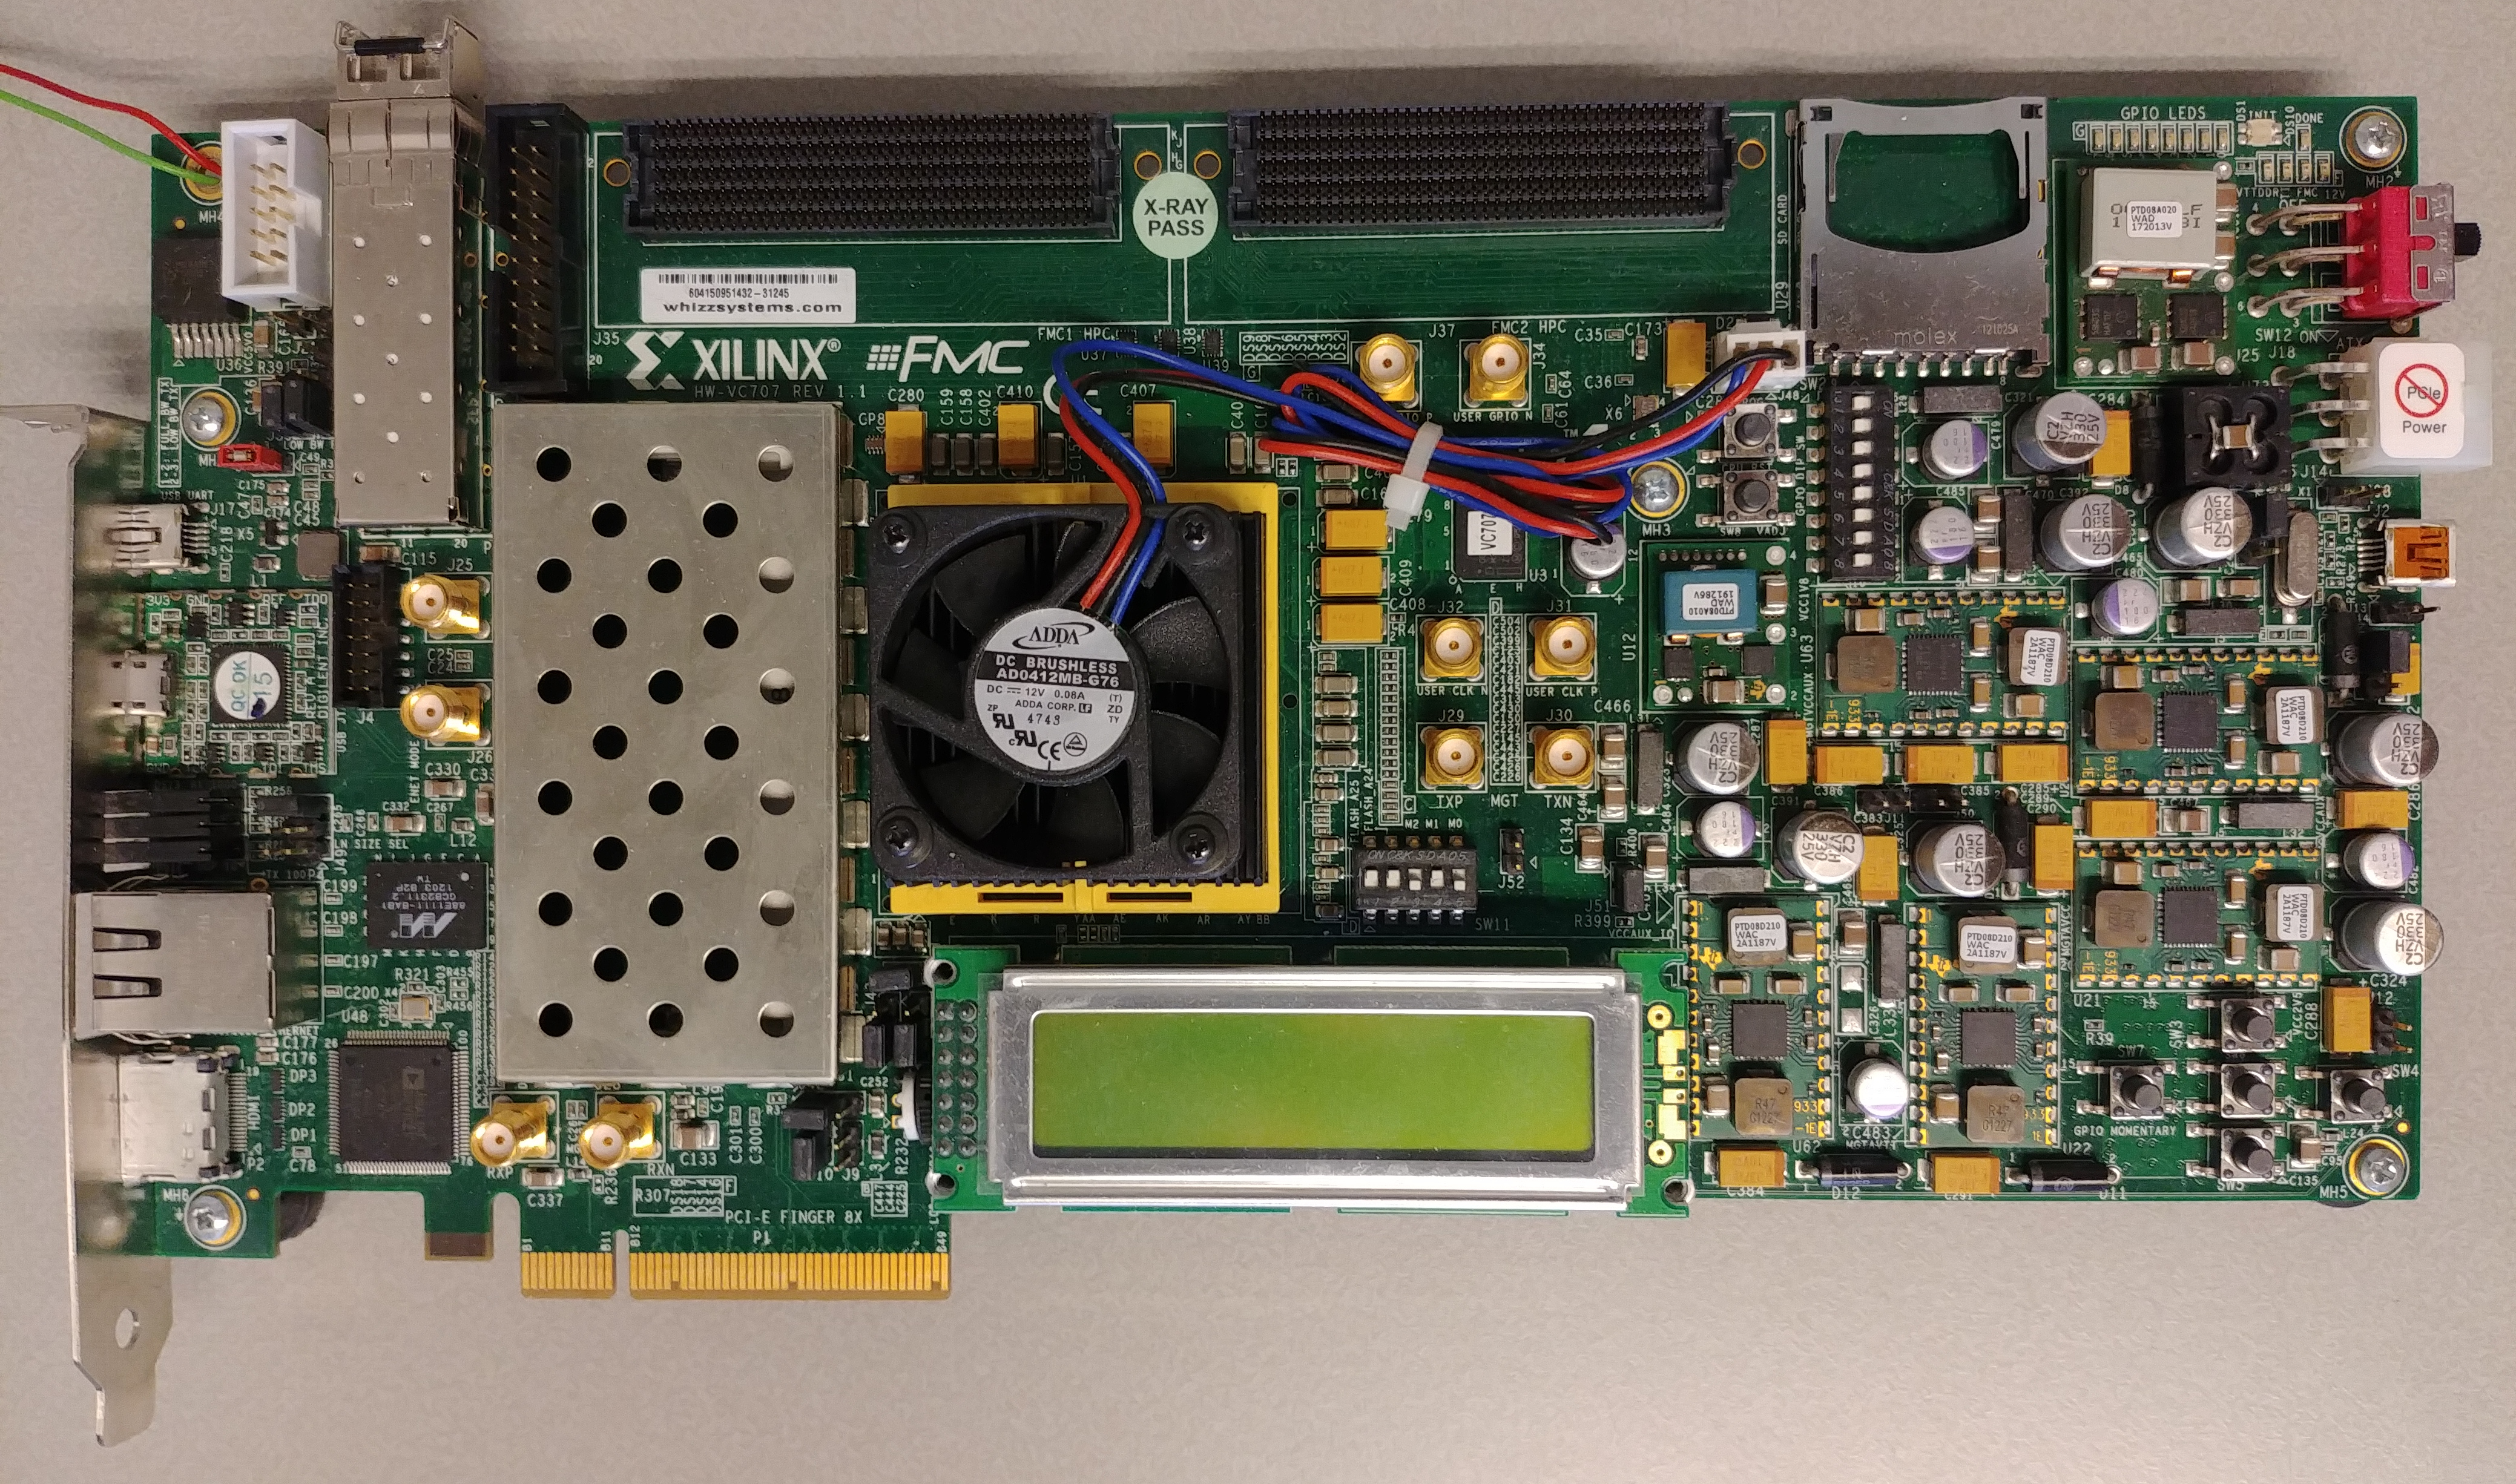
\includegraphics[width=\textwidth]{VC707_Nikhef.jpg}	
	\caption{The Virtex-7 VC707 Board provided by Nikhef.}
	\label{Fig:VC707_Nikhef}
\end{figure}

%The VC707 features a Virtex-7 XC7VX485T-2FFG1761C \cite{Virtex-7} which contains about 486k logic cells and 37 kb ram. The board also features among others 1 GB DDR3, 128 MB Flash, USB 2.0 ULPI transceiver, GTX transceivers, 10/100/1000 tri-speed Ethernet PHY, HDMI codec, PCI Express lanes (Gen 1 x8 \& 2 x8) and SFP+ connector. 

The VC707 Evaluation Board contains 27 accessible GTX transceivers according to the documentation. Eight are wired to the PCI Express x8 connector and sixteen are connected to the FMC connectors. This results in three left from which one is wired to the SMA connectors, another one is connected to the SFP/SFP+ connector and the last one is used in combination with the Ethernet PHY for SGMII connection.

This makes clear that only two of these GTX transceivers are immediately accessible for communication with other boards or products. These are the transceivers wired to the SMA and SFP+ connectors. 

The included GTX transceivers support transfer speeds up to 12,5 Gbps in case the QPLL is used instead of the CPLL, which is excellent since 10 Gbps is the target line rate~\cite{GTXT}. The difference between PLL types and which clocks they generate will be explained in section \ref{subsec:Hardware_Transceiver}. It is even specifically mentioned that in case of Interlaken a line rate of 10,3125 Gbps would be supported. The QPLL frequency would of course be 10,3125 GHz since all data will be serialized and transmitted over the line.

This Chapter will contain separate sections describing the transmitter, receiver and transceiver parts. In case IP cores are used this will be noted with the accompanying version and vendor.
%while the reference clock should be 161,13 MHz. This is understandable since the 10,3125 GHz is a serial transmission and when this is converted to a parallel bus the same speed has to be maintained. This can be calculated dividing 10,3125 GHz by the 64-bits which indeed results in the 161,13 MHz.

\subsection{Transmitter side}
	The transmitter side will be described and designed first. This will deliver more insight in the framing and encoding of the data which will make it easier to remove the framing and decode the transmitted data at the receiving side.
	
	Figure \ref{Fig:Hardware_TX} depicts the complete transmitter side of the interface. Only useful data will be stored and the FIFO can also indicate it is full to other logic. Framing components have to communicate with each other because of the extra space required in between the data flowing. 
	\begin{figure}[H]
		\centering
		\includegraphics[width=\textwidth]{Hardware_TX.png}	
		\caption{Overview of the TX block diagram.}
		\label{Fig:Hardware_TX}
	\end{figure}
	
	\subsubsection[TX FIFO]{TX FIFO \hfill OSI Layer 2}
		The FIFO will act as a buffer temporary storing data when frames are added or the interface can process no more data. It is also especially useful in case the interface needs some extra time before the next frame can be processed. This will often occur during the addition of burst and meta frames.
		
		Another very useful feature of the FIFO is the ability to cross clock domains. Data will be written in the FIFO at a by the user determined rate while to FIFO will be read at the maximum speed the transceiver allows to always keep the line and logic alive/busy.
		
		A separate input port is available to the user which enables the write ability of the FIFO. So only data the user really want to be stored will enter the FIFO. Besides this other control signals like the SOP, EOP and EOP valid will be put together with the data in one signal. The single 68-bit variable will then enter the FIFO.
		
		In case the bursts will be generated according to the optional scheduling enhancement, an extra feature will be required to read the amount of data already placed in the FIFO.\\
		
		The most recent version implements the Xilinx FIFO generator 13.1 IP core.
		
	\subsubsection[Bursts]{Bursts \hfill OSI Layer 2}
		Data leaving the FIFO will be converted to complete bursts. The control signal provided by the user which will leave the FIFO with the data, will be read and according to this the bursts will be formed. Then for example an SOP or EOP burst control word can be generated.
		
		In the Burst component a state machine can be found which remains in idle state unless the burst is enabled and a start of packet is detected. This will trigger the state machine and the arriving data from the FIFO will be read. The data will be saved in several pipelined registers to make packing the data in burst words possible. As explained in Section~\ref{subsec:interlaken_bursts} a burst control word has to be added first. After this the data will follow and as long as the state machine doesn't detect an EOP this continues. Every word of data processed will also cause an increment by one in the word counter because of the maximum burst length, BurstMax, that is allowed. When this value is reached the state machine will switch to another state for one cycle and will return to processing the data again. This has been done so a burst control word can be transmitted between bursts of maximum lengths.
		
		When an EOP signal is detected the state machine will switch to another state. Reading the FIFO will be stopped and a control word which contains the EOP and CRC-24 will follow at the output. After this it is important to check the word counter value. When the data length transmitted in this situation is shorter than the predefined BurstShort, the control word will be followed by one of multiple idle words until the transmitted data length is equal to BurstShort and the state machine will again wait for an SOP signal. In case the transmission contained an amount of words in between the values of BurstShort and BurstMax, no idle words will be necessary to include. 
		
		There is also a situation possible where the user sends data at a slower rate than the complete interface can process. In this case the FIFO will transmit multiple empty flags during transmission. But the transceiver is still expecting data so the empty spaces are filled up with idle words. This way data is still transmitted and the link is kept alive. In case these idle words won't be used, the FIFO will still output the last value in it's memory. The interface will then just processes this as useful data which results in duplicated data at the receiving side. Plus an RX FIFO overflow since the RX FIFO will be read at the same rate the TX FIFO is filled.\\
		
		An implementation of the optional scheduling enhancement is recommended but not yet developed.
		 
	\subsubsection[Meta Frame]{Meta Framing \hfill OSI Layer 2}
		This component will add the meta frames to the data transmission, as discussed in section~\ref{subsec:interlaken_metaframe} this will be four words. It contains a state machine that counts the passed data words. When the transmission starts, these four control words will appear at the output. During these four cycles data will be read and pipelined so when the control words have passed, data will immediately follow. When the word length of the passed data reaches a value of MetaFrameLength, including the several data words, the state will change.
		
		Firstly the pipelined data will be output so it takes several cycles before all data left the component. After this the framing words will be output again to complete the meta frame and during this process input data will already enter the pipeline registers again. This way the cycle repeats and a complete meta frame will always appear at the output. One last thing to consider is the FIFO will also stop being read for four clock cycles. Otherwise there won't be place for the framing words.
		
	\subsubsection[CRC generation]{Generating CRC \hfill OSI Layer 2}
		Bursts and Meta Frames both contain variants of the CRC and generating this will be explained in this subsection. Both contain the same method since they will check a certain length of words and also the specific word that will contain the CRC itself later.
		
		The component responsible for generating the CRC needs two clock cycles to let this check appear at the output. In this case a method is used where data enters the CRC component but is also saved in original state parallel to the register because this has yet to be transmitted. Since the control words containing the reserved space for the CRC also have to be checked, the data has actually to be held in parallel registers for two clock cycles. This method makes it fairly simple to put the generated CRC in the control word since this word and the CRC now are available on the same clock cycle. Now it's just a matter of moving the bits to the right position in the control word.
		Figure~\ref{Fig:Hardware_CRC} shows a visual representation of this.
		\begin{figure}[H]
			\centering
			\includegraphics[width=0.6\textwidth]{Hardware_CRC.png}	
			\caption{Used method generating CRC.}
			\label{Fig:Hardware_CRC}
		\end{figure}
		
	\subsubsection[Scrambler]{Scrambler \hfill OSI Layer 1}
		The scrambler will receive a 64-bit data input from the meta framing component. Since the synchronization and scrambler state words won't have to be scrambled these have to be detected first. When the control input signal is low this means data is entering the scrambler and this will always be scrambled. In case the control input is high this first six bits will be looked at. This way the scrambler can determine whether the word is synchronization, scrambler state or other control word. The first will leave the scrambler untouched while the second will appear at the output after the current scrambler state has been added to the word. All other control words will be scrambled. The scrambled data will be outputted alongside the control word indicator and a data valid signal.
		
		The scrambler polynomial has been defined before. The Interlaken Protocol Definition already includes a piece of code in Appendix B showing how to constantly generate the output and new state of the polynomial. This code was unfortunately written in Verilog so only the part generating the polynomial has been used and was translated to VHDL.

	\subsubsection[Encoder]{Encoder \hfill OSI Layer 1}
		The encoder will accept the scrambled data output. When enabled all data packets will be added a 3-bit preamble header. The control word input signal will indicate what the first two preamble bits accompanying the word should be. When the word is data '01' will be added and when a control word appears this will be '10'.
		
		For the determination of the inversion bit a separate variable will be reset every clock cycle. This will count the running disparity of the incoming data using a for-loop. The value will be saved and compared to the running disparity value of the data just being transmitted. This data is located in a separate variable. 
		
		In case both words contain a majority of the same symbol, the bits of the incoming data will be inverted and the inversion bit will be added to the preamble as a logic high. After this the data will be moved to another variable and will this time be compared to the newly appearing input concerning running disparity.
		
		After this process a 67-bit word will leave the encoder and should be ready for transmission. The transceiver will accept this data and is responsible for the real transmission.

\newpage
\subsection{Receiver side}
	The receiving side will be responsible for restoring the data to its original form before this entered the interface. During development of the transmitter side many knowledge has been gained which makes it easier to develop the receiver side. While the transmitting side added framing words and encoded data, the receiving side has to decode this again and remove the frames. Figure \ref{Fig:Hardware_RX} depicts an overview of the receiver side.
	
	\begin{figure}[H]
		\centering
		\includegraphics[width=\textwidth]{Hardware_RX.png}	
		\caption{Overview of the RX block diagram.}
		\label{Fig:Hardware_RX}
	\end{figure}
	
	\subsubsection[RX FIFO]{RX FIFO \hfill OSI Layer 2}
		The original data identical to the data before entering the interface will be written in this FIFO. Again it is also used to cross clock domains since the interface itself will be running at a standard frequency but the user clock may vary or configure at a different frequency. 
		
		Only when the component removing the burst frames output a valid signal, the data appearing at the FIFO input will be stored. Otherwise the data will be ignored since it then concerns a control word or duplicated data which is not useful. This means the valid signal is connected to the FIFO write enable pin.
		
		The user has to set the FIFO read signal high before any data will appear at the output which prevents data loss. In case the user logic is busy with other tasks and can't process the data, this will remain stored in the FIFO. However the chance on the FIFO overflowing is fairly high in such situating. This will be prevented by flow control which will be discussed in \ref{subsec:Hardware_FlowControl}. For this the FIFO programmable full signal can be used which offers a set value and threshold based on how far the FIFO is filled with data.\\ 
		
		The most recent version implements the Xilinx FIFO generator 13.1 IP core.
	
	\subsubsection[Deframing Burst]{Deframing Burst \hfill OSI Layer 2}
		The added burst control words have to be removed. However these words contain critical information which have to be read and processed before simply deleting words. For example in case an SOP or EOP is detected, the user interface will output a high SOP or EOP pin.
		
		The deframing can easily be done by inspecting the valid and control indicator which accompany each word. When the valid signal is low the data will simply be ignored. In case valid is high and control is also high, this indicates a valid burst control word. Since different burst control words each contain other viable information, it will first be determined which word this is. According to this analysis the useful information will be extracted. This data will be saved and appear at the output accompanying the next data word. For example an SOP be added to the next word. One exception is the EOP since this actually has to accompany the most recent passed data word.
		
		In case valid is high and control low, the entering word will be considered as valid data. However this data will not yet appear at the output but is saved. This is done because an EOP can follow anytime and in case the data word is released to early the EOP will miss. When another valid data or control word enters the component, the saved word will be released. This means the possible appeared EOP or earlier SOP will appear at the output of the component together with the data.
		
		Another valid signal at the output will switch to high when the data leaves the component to indicate the FIFO that this data is useful and has to be stored.
		
	\subsubsection[Deframing Meta]{Deframing Meta \hfill OSI Layer 2}
		The meta frames are useful during transmission and deframing but they have to be invalidated in the process of outputting only the original user data. The descrambler uses these frames to synchronize itself and before deframing the CRC-32 has also to be checked. 
		After this the meta frames will simply be ignored by making their accompanying valid signal low at the output. This way other components will just ignore them. Of course when data enters this component with a logical low accompanying valid signal, the data will be ignored.
		
	\subsubsection[CRC checking]{CRC checking \hfill OSI Layer 2}
		Error checking will be done generating the CRC again like at the transmitter side. This generated value will be compared to the received CRC value in the control words. In case these match the data arrived flawless. When these don't match data corruption occurred and the data is not identical to that at the transmitting side.

	\subsubsection[Descrambler]{Descrambler \hfill OSI Layer 1}
		Data leaving the decoder is still in scrambled format and not yes usable. When starting the descrambler it won't process any input data but instead look for the unscrambled synchronization words. The control words indicator from the decoder will be read. In case this indicates a control word and the block type is identical to the synchronization one, the data will be compared to the predefined sync data. In case these are identical, the state machine will move into another state and two counters start. In case the input data valid signal is a logical low, this word will be ignored so the scrambler state will also not change.
		
		The amount of passing words will be counted. After a certain MetaFrameLength amount of words the synchronization word has to appear again. In case this happens the sync word counter will be incremented by one. In case this reaches the value of four, the state machine moves to the next state indicating a lock.
		
		When in lock all words at the input will be descrambled, except the sync and scrambler state words of course. There will still be checked on correct synchronization words and in case this is not identical to the word expected, the sync word error counter will be incremented by one. After this the scrambler state word is expected to arrive. In case this matches the current polynomial the status should remain locked. Otherwise the scrambler state mismatch counter will increment by one. 
		
		When the sync word error or the scrambler state mismatch counters reaches the value of respectively four or three, a reset will follow. The descrambler loses its lock and has to look for synchronization words again to get in lock.
		
	\subsubsection[Decoder]{Decoder \hfill OSI Layer 1}
		The decoder will immediately receive data from the transceiver. Thus data entering the decoder will be 67-bit wide. This part will be responsible for removing the preamble and reducing the data width to 64-bits. The scrambled data will remain to be descrambled and the preamble will be converted to a separate control word indicator. The inversion bit in the preamble will be read and according to this data will be inverted or not, then the inversion bit will be discarded.
		
		One of the most important functions of the decoder is to alight the data correctly. Since the data is scrambled and cannot be read, the preamble has to be used for alignment. The decoder can lock on the bit transition in the preamble which assures the 64-bits leaving the decoder are really identical to the packet that has been transmitted. 
		
		In combination with the transceiver from Xilinx, the decoder can use a separate pin for bit slipping. This will cause the transceiver to change the alignment of data during data processing and changes the preamble position. After every bit slip operation the current location of the preamble will be checked and when this is not located at the last three bits, the slip operation will repeat until the preamble is at the right location. This will also cause the decoder to go into lock after 64 consecutive words contain the right preamble location.
		
		When in lock the amount of processed words will be tracked by using a counter. A single word that is not correctly synchronized will not immediately cause the decoder to lose lock. For this an error counter is used which will keep track of the incorrectly synced words. After sixteen errors the decoder will lose lock and reset. This is determined over all words processed but every 64 words. After these 64 words the word counter and error status will be reset. Fortunately the three preamble bits only effectively use 50\% of the valid conditions so errors should not be common and will be easily detected.
		
		The implemented decoder contains three outputs. Two are for the control and valid signals while another one is of course for the data/control word itself. This makes it easy for the components after this to know which type of data this 64-bit word is.
		
\subsection[Flow control]{Flow control \hfill OSI Layer 2}
	\label{subsec:Hardware_FlowControl}
	It is of great importance to constantly check the RX FIFO status. It can be that the user logic reading the FIFO is busy and cannot keep up with the link speed. In case overflows normally start to occur, data will be lost permanently and this may not be allowed to happen. The solution to this problem is to let the receiver constantly check the RX FIFO status. When the FIFO start filling up more than usual and begins to have a tendency to overflow, there will be a signal generated that will cause the control words to transmit an XOFF for the specific channel. 
	When the side responsible for transmitting the side receives this message, action will be taken by stopping to read the TX FIFO. This way the TX FIFO will fill up somewhat more and the FIFO will update the user logic on this which will stop sending data.
		

\subsection{Transceiver}
	\label{subsec:Hardware_Transceiver}
	Separate hardware is required to set up the 10 Gbps link itself. For such link a 10 GHz clock signal is required and of course the parallel data should be serialized to ready it for serial transmission. A great thing is that the transceiver already takes care of this. The only requirements are to configure it correctly and to provide stable clocks.
	
	Because a Xilinx FPGA is used for testing, the Xilinx transceiver will also be used. This will of course have consequences for the whole core being FPGA vendor independent but in this case there is no other solution. 
	
	The GTX transceiver in the Virtex-7 contains two types of PLL's (Phase Locked Loops) which generates the clock frequency required for the transmission line. In this case the QPLL will be used since the CPLL is limited at a lower maximum frequency and is less stable. The transceiver connected to the SFP+ connection will be used to transmit the data over fiber. The accompanying GTX transceiver is located at Quad0 and is noted as GTX\_X1Y2. The clock the Interlaken Interface itself works on is expected to be $10,0 Gbit / 64 bits = 156,25 MHz$.
	
	During startup the transceiver needs several microseconds to configure itself and to lock the QPLL. After this data can be applied to get the other part of the interface locked.
	
	The transceiver also requires a 40 MHz DRP clock which will be generated with the Xilinx Clocking Wizard 5.3 IP core. The most recent version implements the Xilinx Transceiver Wizard 3.6 IP core.

\subsection{Complete interface}
	When all components are combined to one complete interface the overview should look like depicted in \ref{Fig:Core1990}. This includes the transmitter and receiver logic connected to the transceiver. While the interface only requires the user to input data and control signals with it, certain clocks should of course also be provided. The complete core that has been developed will be accompanied by it's own documentation which will be described in Appendix \ref{Appendix:Core1990}.
	
	\begin{figure}[H]
		\centering
		\includegraphics[width=\textwidth]{Core1990_Overview.png}	
		\caption{Complete Core1990 architecture.}
		\label{Fig:Core1990}
	\end{figure}

\newpage